\documentclass[twoside]{book}

% Packages required by doxygen
\usepackage{calc}
\usepackage{doxygen}
\usepackage{graphicx}
\usepackage[utf8]{inputenc}
\usepackage{makeidx}
\usepackage{multicol}
\usepackage{multirow}
\usepackage{textcomp}
\usepackage[table]{xcolor}

% Font selection
\usepackage[T1]{fontenc}
\usepackage{mathptmx}
\usepackage[scaled=.90]{helvet}
\usepackage{courier}
\usepackage{amssymb}
\usepackage{sectsty}
\renewcommand{\familydefault}{\sfdefault}
\allsectionsfont{%
  \fontseries{bc}\selectfont%
  \color{darkgray}%
}
\renewcommand{\DoxyLabelFont}{%
  \fontseries{bc}\selectfont%
  \color{darkgray}%
}

% Page & text layout
\usepackage{geometry}
\geometry{%
  a4paper,%
  top=2.5cm,%
  bottom=2.5cm,%
  left=2.5cm,%
  right=2.5cm%
}
\tolerance=750
\hfuzz=15pt
\hbadness=750
\setlength{\emergencystretch}{15pt}
\setlength{\parindent}{0cm}
\setlength{\parskip}{0.2cm}
\makeatletter
\renewcommand{\paragraph}{%
  \@startsection{paragraph}{4}{0ex}{-1.0ex}{1.0ex}{%
    \normalfont\normalsize\bfseries\SS@parafont%
  }%
}
\renewcommand{\subparagraph}{%
  \@startsection{subparagraph}{5}{0ex}{-1.0ex}{1.0ex}{%
    \normalfont\normalsize\bfseries\SS@subparafont%
  }%
}
\makeatother

% Headers & footers
\usepackage{fancyhdr}
\pagestyle{fancyplain}
\fancyhead[LE]{\fancyplain{}{\bfseries\thepage}}
\fancyhead[CE]{\fancyplain{}{}}
\fancyhead[RE]{\fancyplain{}{\bfseries\leftmark}}
\fancyhead[LO]{\fancyplain{}{\bfseries\rightmark}}
\fancyhead[CO]{\fancyplain{}{}}
\fancyhead[RO]{\fancyplain{}{\bfseries\thepage}}
\fancyfoot[LE]{\fancyplain{}{}}
\fancyfoot[CE]{\fancyplain{}{}}
\fancyfoot[RE]{\fancyplain{}{\bfseries\scriptsize Generated on Sun Sep 7 2014 23\-:38\-:29 for My Project by Doxygen }}
\fancyfoot[LO]{\fancyplain{}{\bfseries\scriptsize Generated on Sun Sep 7 2014 23\-:38\-:29 for My Project by Doxygen }}
\fancyfoot[CO]{\fancyplain{}{}}
\fancyfoot[RO]{\fancyplain{}{}}
\renewcommand{\footrulewidth}{0.4pt}
\renewcommand{\chaptermark}[1]{%
  \markboth{#1}{}%
}
\renewcommand{\sectionmark}[1]{%
  \markright{\thesection\ #1}%
}

% Indices & bibliography
\usepackage{natbib}
\usepackage[titles]{tocloft}
\setcounter{tocdepth}{3}
\setcounter{secnumdepth}{5}
\makeindex

% Hyperlinks (required, but should be loaded last)
\usepackage{ifpdf}
\ifpdf
  \usepackage[pdftex,pagebackref=true]{hyperref}
\else
  \usepackage[ps2pdf,pagebackref=true]{hyperref}
\fi
\hypersetup{%
  colorlinks=true,%
  linkcolor=blue,%
  citecolor=blue,%
  unicode%
}

% Custom commands
\newcommand{\clearemptydoublepage}{%
  \newpage{\pagestyle{empty}\cleardoublepage}%
}


%===== C O N T E N T S =====

\begin{document}

% Titlepage & ToC
\hypersetup{pageanchor=false}
\pagenumbering{roman}
\begin{titlepage}
\vspace*{7cm}
\begin{center}%
{\Large My Project }\\
\vspace*{1cm}
{\large Generated by Doxygen 1.8.6}\\
\vspace*{0.5cm}
{\small Sun Sep 7 2014 23:38:29}\\
\end{center}
\end{titlepage}
\clearemptydoublepage
\tableofcontents
\clearemptydoublepage
\pagenumbering{arabic}
\hypersetup{pageanchor=true}

%--- Begin generated contents ---
\chapter{Hierarchical Index}
\section{Class Hierarchy}
This inheritance list is sorted roughly, but not completely, alphabetically\-:\begin{DoxyCompactList}
\item Node\begin{DoxyCompactList}
\item \contentsline{section}{Simple\-List\-Node}{\pageref{classSimpleListNode}}{}
\end{DoxyCompactList}
\end{DoxyCompactList}

\chapter{Class Index}
\section{Class List}
Here are the classes, structs, unions and interfaces with brief descriptions\-:\begin{DoxyCompactList}
\item\contentsline{section}{\hyperlink{class_binary_tree}{Binary\-Tree} }{\pageref{class_binary_tree}}{}
\item\contentsline{section}{\hyperlink{class_binary_tree_node}{Binary\-Tree\-Node} }{\pageref{class_binary_tree_node}}{}
\item\contentsline{section}{\hyperlink{class_iterator}{Iterator} }{\pageref{class_iterator}}{}
\item\contentsline{section}{\hyperlink{class_node}{Node} }{\pageref{class_node}}{}
\item\contentsline{section}{\hyperlink{class_simple_list_node}{Simple\-List\-Node} \\*The \hyperlink{class_simple_list_node}{Simple\-List\-Node} class. A simple list node is the corresponding node to the data structure \char`\"{}simple linked list\char`\"{} }{\pageref{class_simple_list_node}}{}
\end{DoxyCompactList}

\chapter{Class Documentation}
\hypertarget{classSimpleListNode}{\section{Simple\-List\-Node Class Reference}
\label{classSimpleListNode}\index{Simple\-List\-Node@{Simple\-List\-Node}}
}


The \hyperlink{classSimpleListNode}{Simple\-List\-Node} class. A simple list node is the corresponding node to the data structure \char`\"{}simple linked list\char`\"{}. Method list\-:   set\-Element  get\-Element  set\-Next  get\-Next  set\-Previous  get\-Previous  Atribute list\-:   pointer Node \-\_\-previous  pointer Node \-\_\-next .  




{\ttfamily \#include $<$Simple\-List\-Node.\-h$>$}

Inheritance diagram for Simple\-List\-Node\-:\begin{figure}[H]
\begin{center}
\leavevmode
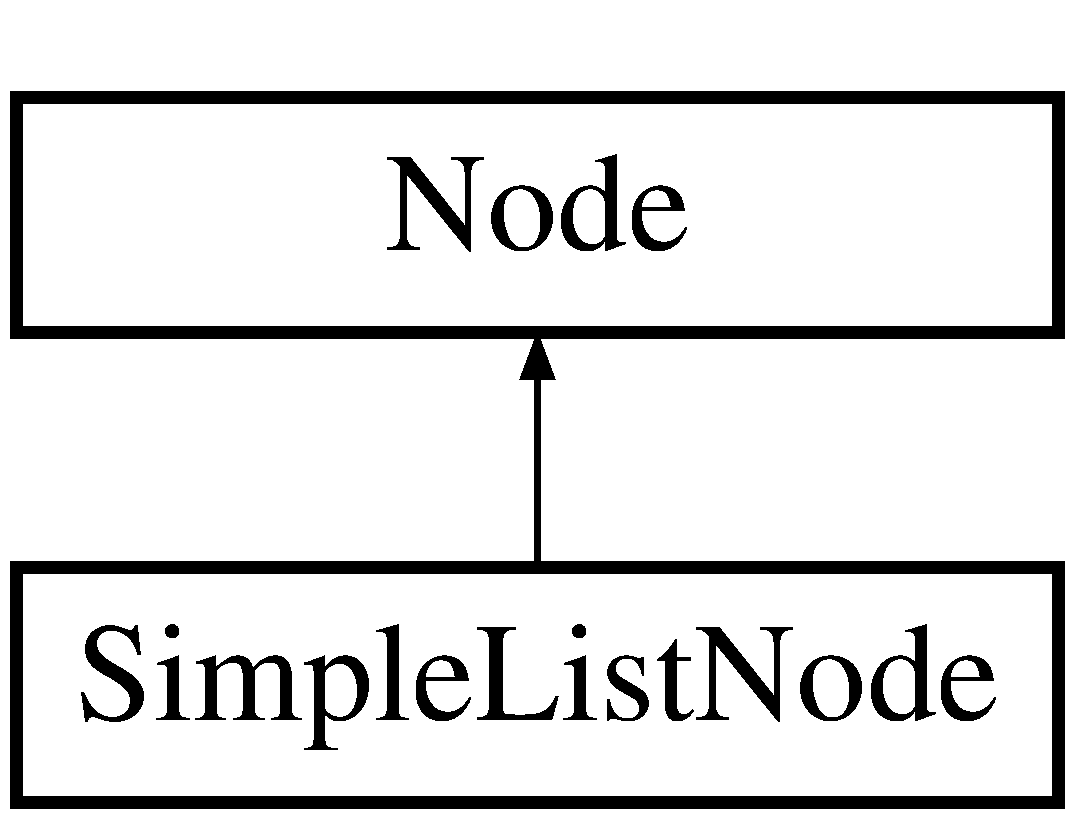
\includegraphics[height=2.000000cm]{classSimpleListNode}
\end{center}
\end{figure}
\subsection*{Public Member Functions}
\begin{DoxyCompactItemize}
\item 
\hypertarget{classSimpleListNode_ad88ea222aee07a6f8b1113c92aa7b069}{void {\bfseries set\-Element} (int p\-Element)}\label{classSimpleListNode_ad88ea222aee07a6f8b1113c92aa7b069}

\item 
\hypertarget{classSimpleListNode_a79a2c3e4610352b4b24de421df8a451d}{int $\ast$ {\bfseries get\-Element} ()}\label{classSimpleListNode_a79a2c3e4610352b4b24de421df8a451d}

\item 
\hypertarget{classSimpleListNode_af36eceb9c6e6cc0d471844d6a952f6cf}{void {\bfseries set\-Next} (\hyperlink{classSimpleListNode}{Simple\-List\-Node} $\ast$p\-Next\-Node)}\label{classSimpleListNode_af36eceb9c6e6cc0d471844d6a952f6cf}

\item 
\hypertarget{classSimpleListNode_a2f2aaa5011673d032ac0e385dc2a4032}{\hyperlink{classSimpleListNode}{Simple\-List\-Node} $\ast$ {\bfseries get\-Next} ()}\label{classSimpleListNode_a2f2aaa5011673d032ac0e385dc2a4032}

\item 
\hypertarget{classSimpleListNode_acebffab49dae4768f695054b0ccff68a}{void {\bfseries set\-Previous} (\hyperlink{classSimpleListNode}{Simple\-List\-Node} $\ast$p\-Previous\-Node)}\label{classSimpleListNode_acebffab49dae4768f695054b0ccff68a}

\item 
\hypertarget{classSimpleListNode_ac4bead7a1bd4e896f8a8e7a8a53cbc3d}{\hyperlink{classSimpleListNode}{Simple\-List\-Node} $\ast$ {\bfseries get\-Previous} ()}\label{classSimpleListNode_ac4bead7a1bd4e896f8a8e7a8a53cbc3d}

\end{DoxyCompactItemize}


\subsection{Detailed Description}
The \hyperlink{classSimpleListNode}{Simple\-List\-Node} class. A simple list node is the corresponding node to the data structure \char`\"{}simple linked list\char`\"{}. Method list\-:   set\-Element  get\-Element  set\-Next  get\-Next  set\-Previous  get\-Previous  Atribute list\-:   pointer Node \-\_\-previous  pointer Node \-\_\-next . 

The documentation for this class was generated from the following files\-:\begin{DoxyCompactItemize}
\item 
Simple\-List\-Node.\-h\item 
Simple\-List\-Node.\-cpp\end{DoxyCompactItemize}

%--- End generated contents ---

% Index
\newpage
\phantomsection
\addcontentsline{toc}{chapter}{Index}
\printindex

\end{document}
